% !TeX program = xelatex
\documentclass[
  convert={density=500, size=600, outext=.png}, 
  border=2pt
]{standalone}

\usepackage{fontspec}
\defaultfontfeatures{Ligatures={NoCommon,%
			NoDiscretionary,%
			NoHistoric,%
			NoRequired,%
			NoContextual}}
\setsansfont{Carlito}[%
	SmallCapsFeatures={Letters=SmallCaps},%
	SmallCapsFont={Roboto},%
	ItalicFeatures={SmallCapsFont=Roboto-Italic},%
	BoldFeatures={SmallCapsFont=Roboto-Bold},%
	BoldItalicFeatures={SmallCapsFont=Roboto-BoldItalic}%
]

\usepackage{tikz}
\usepackage{tikz-cd}
\usetikzlibrary{%
	calc,%
	arrows.meta,%
	arrows,%
	automata,%
	overlay-beamer-styles,%
	snakes,%
	shapes.arrows,%
	shapes.geometric,%
	shapes.symbols,%
	fit,%
	positioning,%
	decorations.pathreplacing,%
	backgrounds,%
}
\tikzset{
	>=Triangle,%
	nodes={align=center},%
	comp/.style={%
			draw,%
			rectangle,%
			very thick,%
			rounded corners,%
			minimum width=2.5cm,%
			minimum height=1cm,%
			fill=white},%
	input/.style={draw,%
			rectangle,%
			thick,%
			minimum width=2.5cm,%
			minimum height=1cm,%
			fill=white},%
	classnode/.style={%
			fill=cgreenlight,%
			rectangle,%
			draw,%
			inner xsep=0},%
	interfacenode/.style={%
			fill=corangelight,%
			rectangle,%
			draw,%
			inner xsep=0},%
	abstractclassnode/.style={%
			fill=cbluelight,%
			rectangle,%
			draw,%
			inner xsep=0},%
	inlinenode/.style={%
			inner xsep=.5cm,%
			minimum height=.6cm},%
}

\definecolor{reddy}{RGB}{172, 0, 51}
\definecolor{dkred}{rgb}{.6, 0, 0}
\definecolor{dkgreen}{rgb}{0, .5, 0}
\definecolor{dkblue}{rgb}{0, 0, .5}
\definecolor{cred}{RGB}{219, 68, 55}
\definecolor{credlight}{RGB}{250, 227, 225}
\definecolor{cgreen}{RGB}{3, 148, 77}
\definecolor{cgreenlight}{RGB}{209, 251, 230}
\definecolor{cblue}{RGB}{2, 119, 189}
\definecolor{cbluelight}{RGB}{208, 237, 254}
\definecolor{corange}{RGB}{173, 128, 2}
\definecolor{corangelight}{RGB}{253, 219, 123}
\newcommand{\cblue}[1]{\textcolor{cblue}{#1}}
\newcommand{\bfcblue}[1]{\textcolor{cblue}{\textbf{#1}}}
\newcommand{\cred}[1]{\textcolor{cred}{#1}}
\newcommand{\bfcred}[1]{\textcolor{cred}{\textbf{#1}}}
\newcommand{\cgreen}[1]{\textcolor{cgreen}{#1}}
\newcommand{\bfcgreen}[1]{\textcolor{cgreen}{\textbf{#1}}}
\newcommand{\corange}[1]{\textcolor{corange}{#1}}
\newcommand{\bfcorange}[1]{\textcolor{corange}{\textbf{#1}}}
\newcommand{\interfacename}[1]{\underline{\textbf{\textit{#1}}}}
\newcommand{\absclassname}[1]{\textbf{\textit{#1}}}
\newcommand{\classname}[1]{\textbf{#1}}

\usepackage{amsmath}
\usepackage{amsfonts}
\usepackage{amssymb}

\usepackage{silence}
\WarningsOff*


\begin{document}
\sffamily

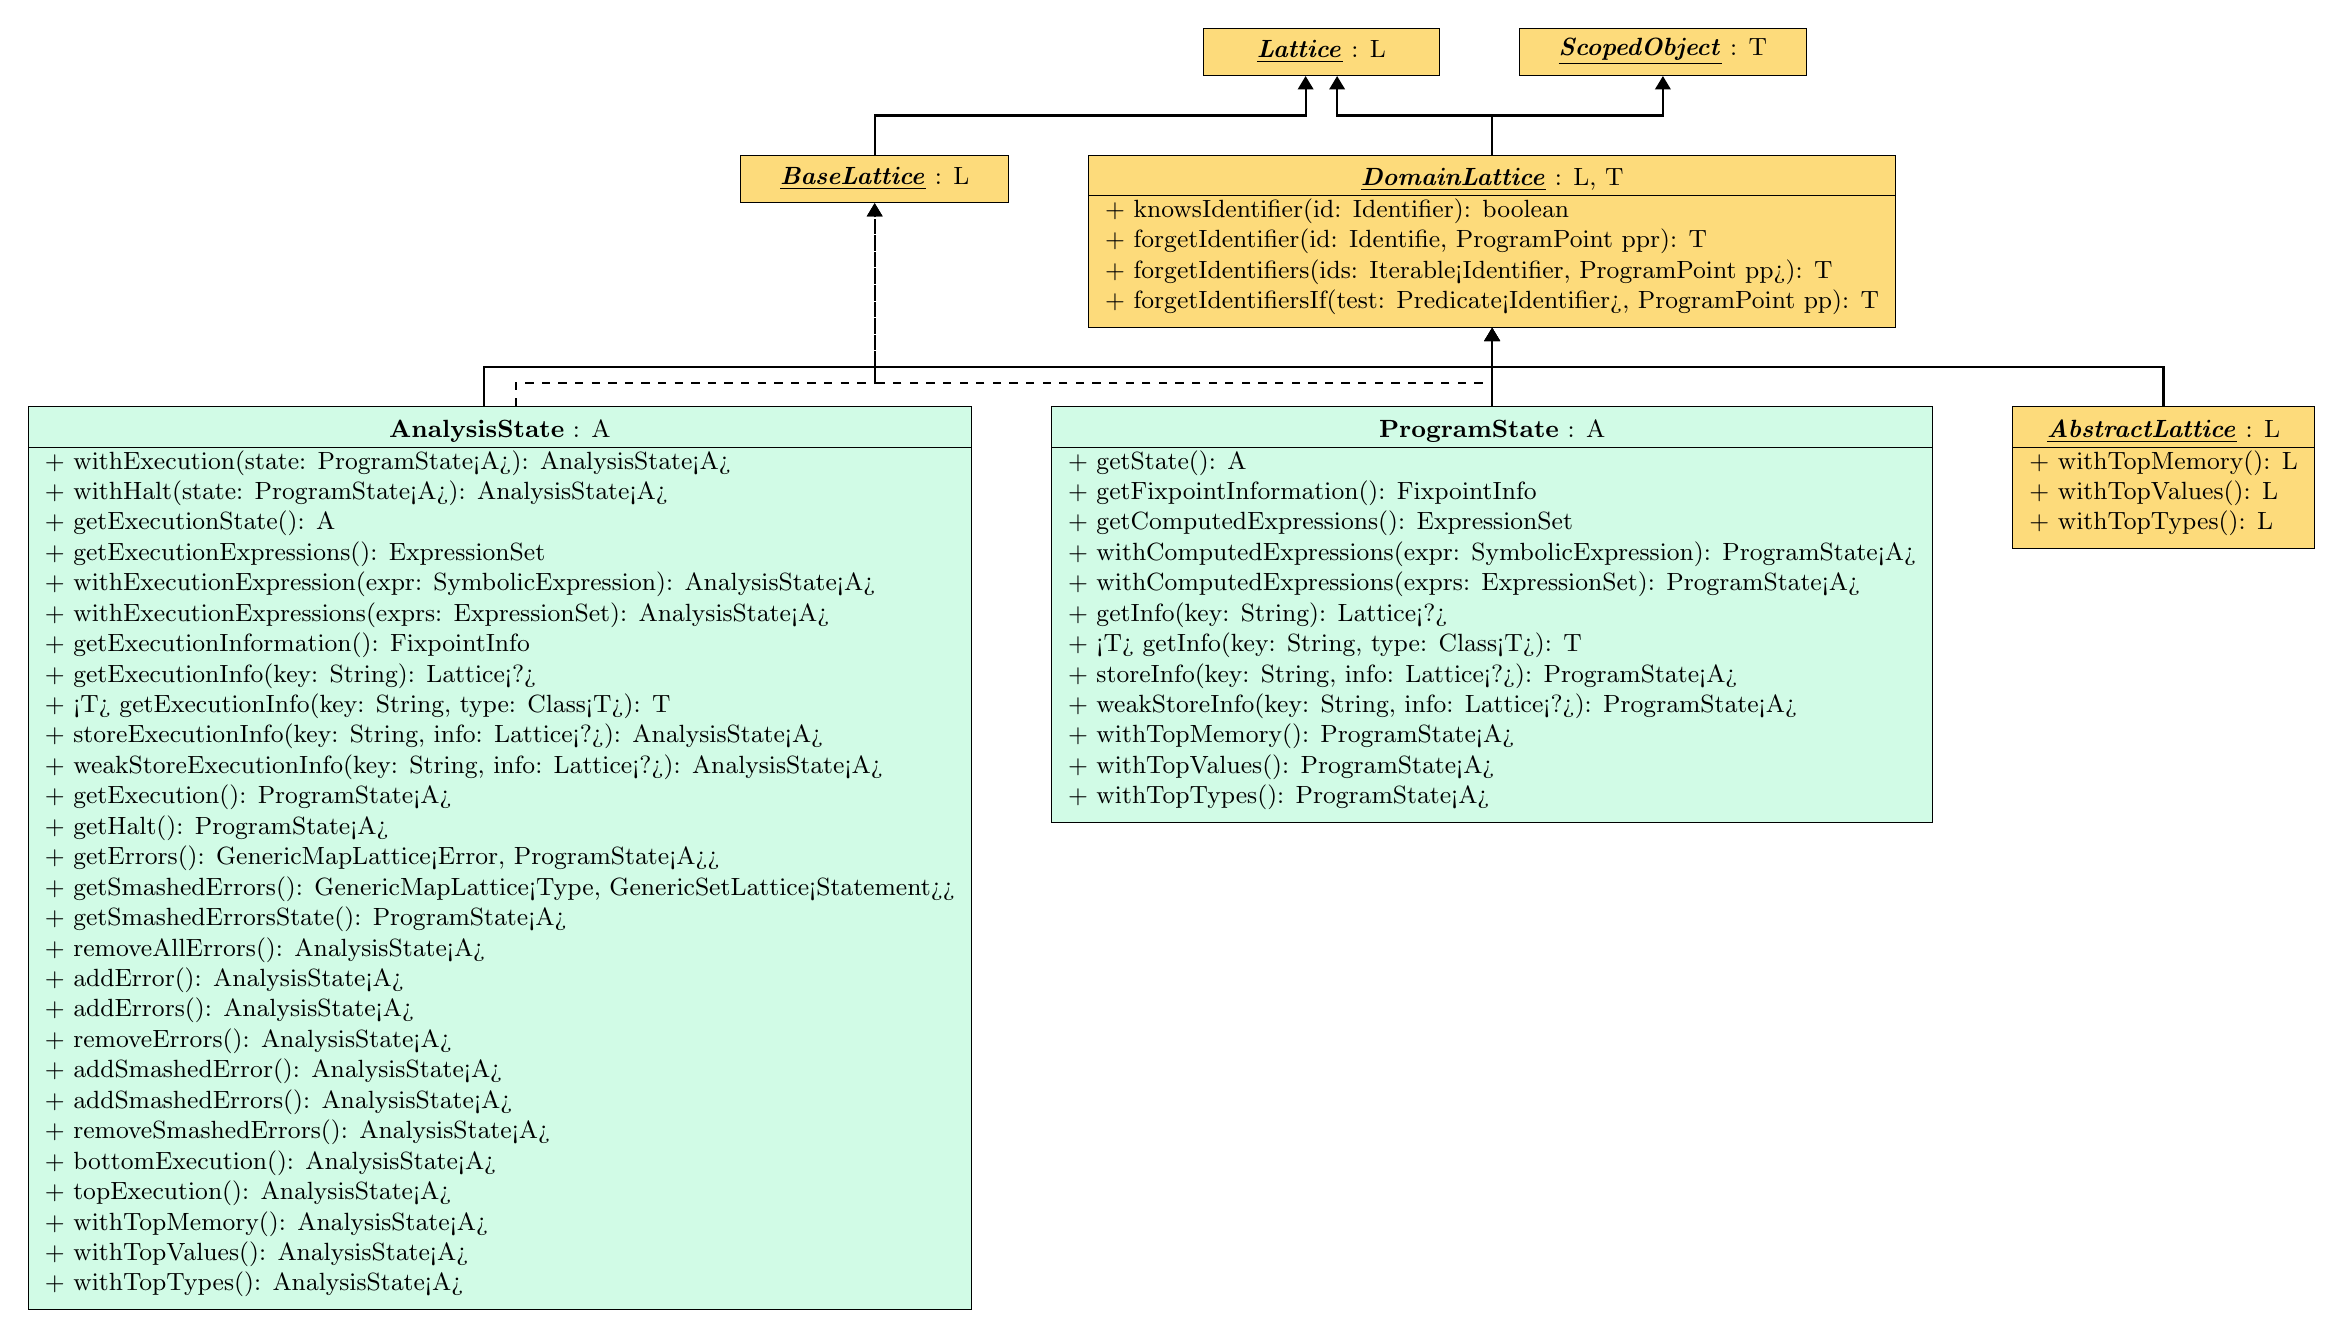
\begin{tikzpicture}[nodes={font={\small}, minimum width=3cm}]%
	\node[interfacenode, inlinenode] (lattice) {\interfacename{Lattice} : L};

	\node[interfacenode, inlinenode] (scoped) [right=of lattice] {\interfacename{ScopedObject} : T};

	\node[interfacenode] (dl) [below=of $(scoped.south)!0.5!(lattice.south)$] {\begin{tabular}{l}
			\multicolumn{1}{c}{\interfacename{DomainLattice} : L, T}               \\
			\hline
			+ knowsIdentifier(id: Identifier): boolean                             \\
			+ forgetIdentifier(id: Identifie, ProgramPoint ppr): T                 \\
			+ forgetIdentifiers(ids: Iterable<Identifier, ProgramPoint pp>): T     \\
			+ forgetIdentifiersIf(test: Predicate<Identifier>, ProgramPoint pp): T \\
		\end{tabular}};

	\node[interfacenode, inlinenode, left=of dl.north west, anchor=north east] (blattice) {\interfacename{BaseLattice} : L};

	\node[classnode] (ps) [below=of dl] {\begin{tabular}{l}
			\multicolumn{1}{c}{\classname{ProgramState} : A}                     \\
			\hline
			+ getState(): A                                                      \\
			+ getFixpointInformation(): FixpointInfo                             \\
			+ getComputedExpressions(): ExpressionSet                            \\
			+ withComputedExpressions(expr: SymbolicExpression): ProgramState<A> \\
			+ withComputedExpressions(exprs: ExpressionSet): ProgramState<A>     \\
			+ getInfo(key: String): Lattice<?>                                   \\
			+ <T> getInfo(key: String, type: Class<T>): T                        \\
			+ storeInfo(key: String, info: Lattice<?>): ProgramState<A>          \\
			+ weakStoreInfo(key: String, info: Lattice<?>): ProgramState<A>      \\
			+ withTopMemory(): ProgramState<A>                                   \\
			+ withTopValues(): ProgramState<A>                                   \\
			+ withTopTypes(): ProgramState<A>                                    \\
		\end{tabular}};

	\node[interfacenode, right=of ps.north east, anchor=north west] (al) {\begin{tabular}{l}
			\multicolumn{1}{c}{\interfacename{AbstractLattice} : L} \\
			\hline
			+ withTopMemory(): L                                    \\
			+ withTopValues(): L                                    \\
			+ withTopTypes(): L                                     \\
		\end{tabular}};

	\node[classnode, left=of ps.north west, anchor=north east] (as) {\begin{tabular}{l}
			\multicolumn{1}{c}{\classname{AnalysisState} : A}                           \\
			\hline
			+ withExecution(state: ProgramState<A>): AnalysisState<A>                   \\
			+ withHalt(state: ProgramState<A>): AnalysisState<A>                        \\
			+ getExecutionState(): A                                                    \\
			+ getExecutionExpressions(): ExpressionSet                                  \\
			+ withExecutionExpression(expr: SymbolicExpression): AnalysisState<A>       \\
			+ withExecutionExpressions(exprs: ExpressionSet): AnalysisState<A>          \\
			+ getExecutionInformation(): FixpointInfo                                   \\
			+ getExecutionInfo(key: String): Lattice<?>                                 \\
			+ <T> getExecutionInfo(key: String, type: Class<T>): T                      \\
			+ storeExecutionInfo(key: String, info: Lattice<?>): AnalysisState<A>       \\
			+ weakStoreExecutionInfo(key: String, info: Lattice<?>): AnalysisState<A>   \\
			+ getExecution(): ProgramState<A>                                           \\
			+ getHalt(): ProgramState<A>                                                \\
			+ getErrors(): GenericMapLattice<Error, ProgramState<A>>                    \\
			+ getSmashedErrors(): GenericMapLattice<Type, GenericSetLattice<Statement>> \\
			+ getSmashedErrorsState(): ProgramState<A>                                  \\
			+ removeAllErrors(): AnalysisState<A>                                       \\
			+ addError(): AnalysisState<A>                                              \\
			+ addErrors(): AnalysisState<A>                                             \\
			+ removeErrors(): AnalysisState<A>                                          \\
			+ addSmashedError(): AnalysisState<A>                                       \\
			+ addSmashedErrors(): AnalysisState<A>                                      \\
			+ removeSmashedErrors(): AnalysisState<A>                                   \\
			+ bottomExecution(): AnalysisState<A>                                       \\
			+ topExecution(): AnalysisState<A>                                          \\
			+ withTopMemory(): AnalysisState<A>                                         \\
			+ withTopValues(): AnalysisState<A>                                         \\
			+ withTopTypes(): AnalysisState<A>                                          \\
		\end{tabular}};

	\draw[->, thick] (dl) |- ($(scoped.south)+(0,-0.5)$) to (scoped);
	\draw[->, thick] (dl) |- ($(lattice.south)+(0.2,-0.5)$) to ($(lattice.south)+(0.2,0)$);
	\draw[->, thick] (blattice) |- ($(lattice.south)+(-0.2,-0.5)$) to ($(lattice.south)+(-0.2,0)$);
	\draw[->, thick] (ps) to (dl);
	\draw[->, thick] (al) |- ($(dl.south)+(0,-0.5)$) to (dl);
	\draw[->, thick] ($(as.north)+(-0.2,0)$) |- ($(dl.south)+(0,-0.5)$) to (dl);
	\draw[->, thick, dashed] ($(as.north)+(0.2,0)$) to ($(as.north)+(0.2,0.3)$) -| (blattice);
	\draw[->, thick, dashed] (ps) to ($(dl.south)+(0,-0.7)$) -| (blattice);
\end{tikzpicture}

\end{document}
